\documentclass[a4paper,twocolumn]{article}

\usepackage[english]{babel}
\usepackage[utf8]{inputenc}
\usepackage{graphicx}
\usepackage{fullpage}

\makeatletter
\newcommand{\thickhline}{%
    \noalign {\ifnum 0=`}\fi \hrule height 1.1pt
    \futurelet \reserved@a \@xhline
}
\newcommand{\thickerhline}{%
    \noalign {\ifnum 0=`}\fi \hrule height 0.65pt
    \futurelet \reserved@a \@xhline
}
\makeatother

\title{(Dynamic) Neural Module Networks $-$ summary}
\author{Matěj Nikl}

\begin{document}
\maketitle
\noindent
This paper tries to address the task of (visual) question answering. One might try to approach this problem with a single, monolithic, deep NN, which would somehow try to answer all possible questions about all possible images (or \textit{worlds} as they are called in general). Authors of this paper, however, tried to tackle this problem in a different way. Take for example a question ``What is in the sheep's ear?''. It can be broken down into smaller subtasks/processing steps:
    \begin{enumerate}
        \item Find sheep
        \item Find ears
        \item \textit{Intersect} those two locations
        \item Describe what is in the intersection
    \end{enumerate}
Those subtasks arise in every question because of the compositional nature of language.

\begin{figure}[h]
    \centering
    \frame{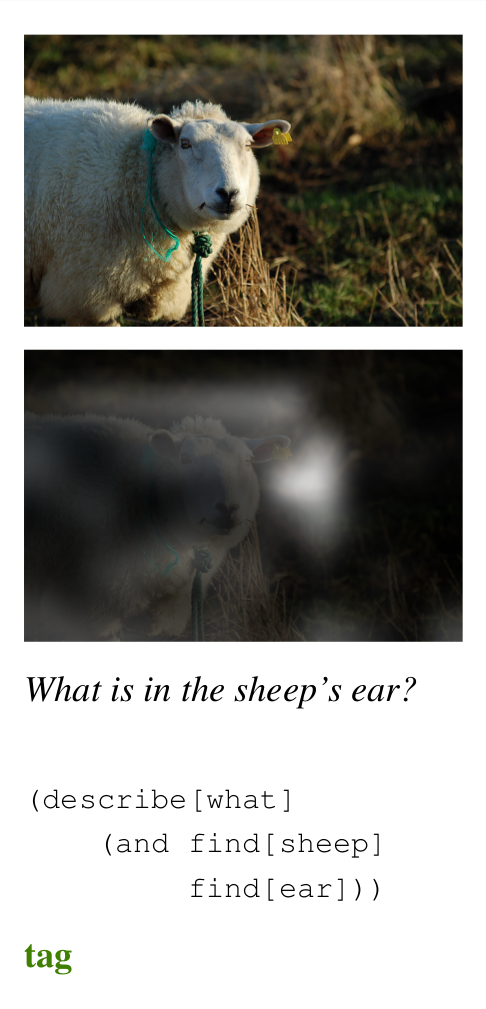
\includegraphics[width=0.35\columnwidth]{sheep.png}}
    \frame{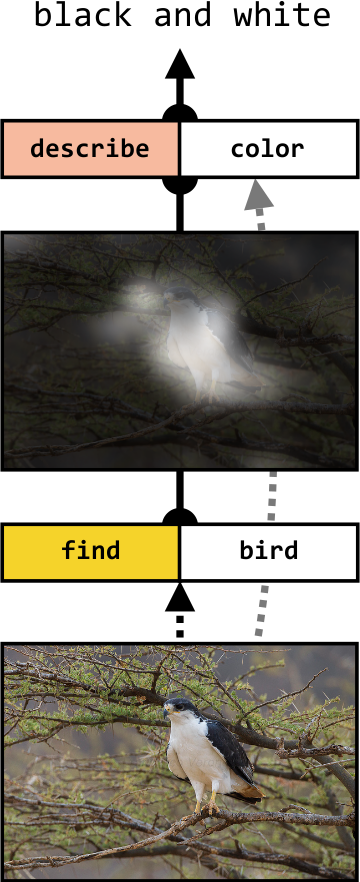
\includegraphics[width=0.35\columnwidth]{bird.png}}
    \caption{Examples of network instances and their computation processes}
\end{figure}

\noindent
Applying these operations would lead to the correct answer. Thus, it was proposed to use such modules that would compute simpler operations and compose them for each question in a way that would lead to a correct answer. This gives a rise to a few more problems to solve:

\subsubsection*{Module types}
It is needed to hand-craft general module types (and their purposes) to fit the needs of the problem given. Following module types were proposed for the task of (V)QA:
    \begin{itemize}
        \item Lookup$[i]$ – produces an attention focused entirely at the index $i$, where the positions in the input map are known ahead of time (e.g. string matches on database fields)
        \item Find$[i]$ – produces an attention map by concatenating $i$ with each position of the input feature map and passing the concatenated vector through a MLP
        \item Relate$[i](h)$ – similar to find, also takes in account current region of attention $h$
        \item And$(h^1, h^2, \dots)$ – perform a \textit{intersect} operation on attention maps (by element-wise multiplication of the attention maps)
        \item Describe$[i](h)$ – predicts a label from a weighted feature vector (with $i$) under the input attention $h$
        \item Exists$(h)$ – existential quantifier examining directly the attention map $h$ to produce a label
    \end{itemize}
They all have their own purposes and might be useful on their own, however their true
power comes when they get arranged to form a tree of operations, applying one after another, performing potentially more and more complex computation with each consecutive processing.

{
\renewcommand{\arraystretch}{1.25}
\begin{table*}[ht]
    \centering
    \begin{tabular}{l c c c c c c}
        \thickhline
        & \multicolumn{4}{c}{test-dev} && test-std \\
        \cline{2-5} \cline{7-5}
        & Yes/No & Number & Other & All && All \\
        \thickerhline
        Zhou (2015) & 76.6 & 35.0 & 42.6 & 55.9 && 55.9 \\
        Noh (2015)  & 80.7 & 37.2 & 41.7 & 57.4 && 57.4 \\
        Yang (2015) & 79.3 & 36.6 & 46.1 & 58.9 && 58.9 \\
        NMN         & 81.2 & 38.0 & 44.0 & 58.7 && 58.7 \\
        D-NMN       & 81.1 & 38.6 & 45.5 & 59.4 && \textbf{59.4} \\
        \thickhline
    \end{tabular}
    \caption{Results on the VQA test server.}
\end{table*}
}

\subsubsection*{Inter-module communication}
In this proposed framework we essentially have 3 types of information flowing in/out of the modules:
    \begin{itemize}
        \item Image (world) data
        \item Attention map
        \item Label
    \end{itemize}
And because different modules might require different types of inputs as well as might produce different types of outputs, they cannot be assembled in all combinations possible. That is, however, not a flaw and it does not impose any practical limitation, because all the meaningful network layouts are possible.

\subsubsection*{Module training}
For each question a network is built and used for a label (answer) prediction.  Since all the modules' operations are differentiable, we can maximize the log-likelihood of the correct answer being produced and back-propagate the error through all modules involved. Because of the dynamic network structures, some modules are used more often then others and their weights are updated more often then others, thus learning algorithms with adaptive per-weight learning rates perform substantially better than simple gradient descent.

% \subsubsection*{How to determine how to arrange those modules into a network so that it would answer the question given?}
\subsubsection*{Assembling a network}
% \subsubsection*{How to create a proper network layout for the question given?}
    The proposed approach is to perform a syntactic parse on the question to generate a small set of layout candidates. To choose the best one, all layouts need to be scored. For that a LSTM representation of the question, as well as a feature-based representation of the layout being scored, are produced and passed through a MLP. The layout feature vector includes indicators of the number of modules of each type present and their arguments (e.g. that a find module is looking for a dog).
 However, choosing the best layout is non-differentiable, thus reinforcement learning needs to be used to train the scoring MLP.

\subsection*{Principles of modularization}
This whole idea is based on modular design with individual modules of several types preforming single \textit{simple} operations, out of which networks are built (into a tree-like structure, where root gives the output) according to the question being asked.

\subsection*{Principles of growing}
Growing is done by attaching individual modules together, achieving a potentially unlimited complexity (to reflect complexity of the given question), however ordinary questions generally require only up to 6 modules to express properly.

\end{document}
